\documentclass[a4paper,12pt]{article}
\usepackage{titlesec}
\titlelabel{\thetitle.\ }
\usepackage{array}
\usepackage{graphicx}
\usepackage{color}
\usepackage{colortbl}
\usepackage[export]{adjustbox}
\usepackage{multirow}
\usepackage{amssymb,amsmath}
\usepackage{hyperref}
\usepackage{empheq}
% \usepackage[most]{tcolorbox}
\usepackage{gensymb}

\usepackage{tikz}
\usepackage{ctable}
\usetikzlibrary{shapes.misc,shadows}

\usepackage{geometry}
 \geometry{
 a4paper,
 total={210mm,297mm},
 left=20mm,
 right=20mm,
 top=16mm,
 bottom=15mm,
 }


\newcommand{\Conv}{%
  \mathop{\scalebox{1.5}{\raisebox{-0.2ex}{$\circledast$}}
  }
}

\newcommand{\Add}{%
  \mathop{\scalebox{1.5}{\raisebox{-0.2ex}{$\oplus$}}
  }
}


\definecolor{myyellow}{rgb}{255, 255, 0}
\newcommand*\myyellowbox[1]{%
% \fcolorbox{black}{myyellow}{\hspace{1em}#1\hspace{1em}}}
\colorbox{myyellow}{\hspace{1em}#1\hspace{1em}}}

\title{A gentle explanation of Backpropagation in Convolutional Neural Network}
\author{Son Nguyen}

\pagestyle{empty}
\begin{document}
\maketitle
Recently, I have read some articles about Convolutional Neural Network, for example, [1], [2], and the notes of the Stanford CS class CS231n [3]. These articles explain Convolutional Neural Network's architecture and its layers very well but they didn't include a detailed explanation of Backpropagation in Convolutional Neural Network. After digging the Internet more deeper and wider, I found two articles [4] and [5] explaining the Backpropagation phase pretty deeply but I feel they are still abstract to me. Because I want a more tangible and detailed explanation so I decided to write this article myself. I hope that it is helpful to you.

\newpage
\section{Prerequisites}
To fully understand this article, I highly recommend you to read the following articles to grasp firmly the foundation of Convolutional Neural Network beforehand:
\begin{itemize}
\item \url{http://cs231n.github.io/convolutional-networks/}
\item \url{https://victorzhou.com/blog/intro-to-cnns-part-1/}
\end{itemize}

\section{Architecture}
In this article, I will build a real Convolutional Neural Network from scratch to classify handwritten digits in the MNIST database provided by \url{http://yann.lecun.com/exdb/mnist/}. At an abstract level, the architecture looks like:
\begin{figure}[h]
  \begin{center}
    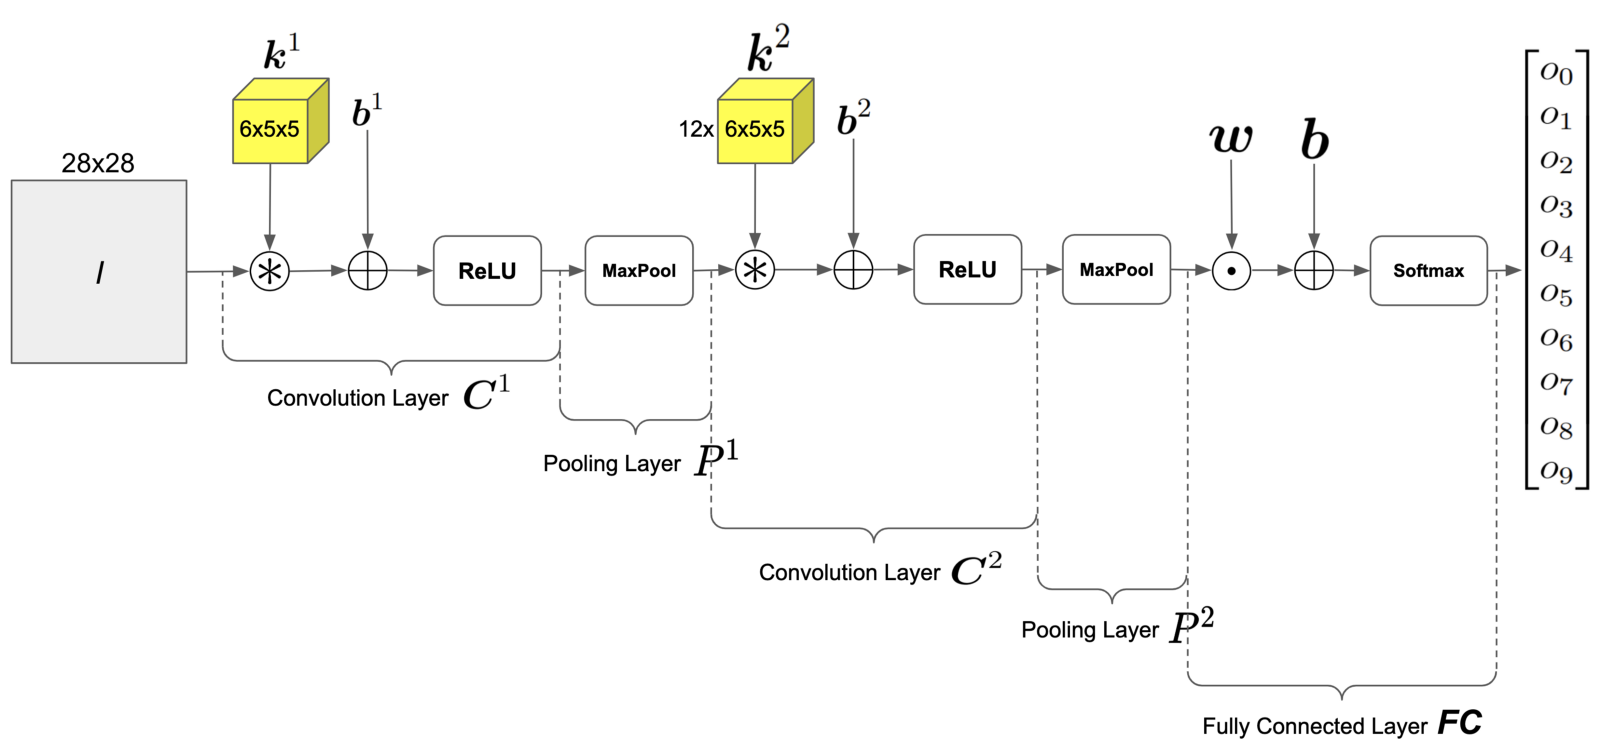
\includegraphics[width=15.6cm, height=7.15cm]{Architecture-abstract.png}
    \caption{Abstract Architecture}
  \end{center}
\end{figure}\\

where 
\begin{itemize}
\item $\boldsymbol{I}$ is a grayscale image with size $28\times28$
\item the kernel $\boldsymbol{k^1}$ is a 3D array with size $6\times5\times5$
\item the bias $\boldsymbol{b^1}$ is a 1D array with size $6$
\item the kernel $\boldsymbol{k^2}$ is a 4D array with size $12\times6\times5\times5$
\item the bias $\boldsymbol{b^2}$ is a 1D array with size $12$
\item the weight $\boldsymbol{w}$ is a 2D array with size $10\times192$
\item the bias $\boldsymbol{b}$ is a 1D array with size $10$
\item the output $\boldsymbol{O}$ is a 1D array with size $10$
\end{itemize}
In the first and second Convolution Layers, I use \textbf{ReLU} functions (Rectified Linear Unit) as activation functions. I use \textbf{MaxPool} with pool size $2\times2$ in the first and second Pooling Layers. And, I use \textbf{Softmax} as an activation function in the Fully Connected Layer.\\
Zooming in the abstract architecture, we will have a detailed architecture split into two following parts (I split the detailed architecture into 2 parts because it's too long to fit on a single page):\\
\\
\begin{figure}[h]
  \begin{center}
    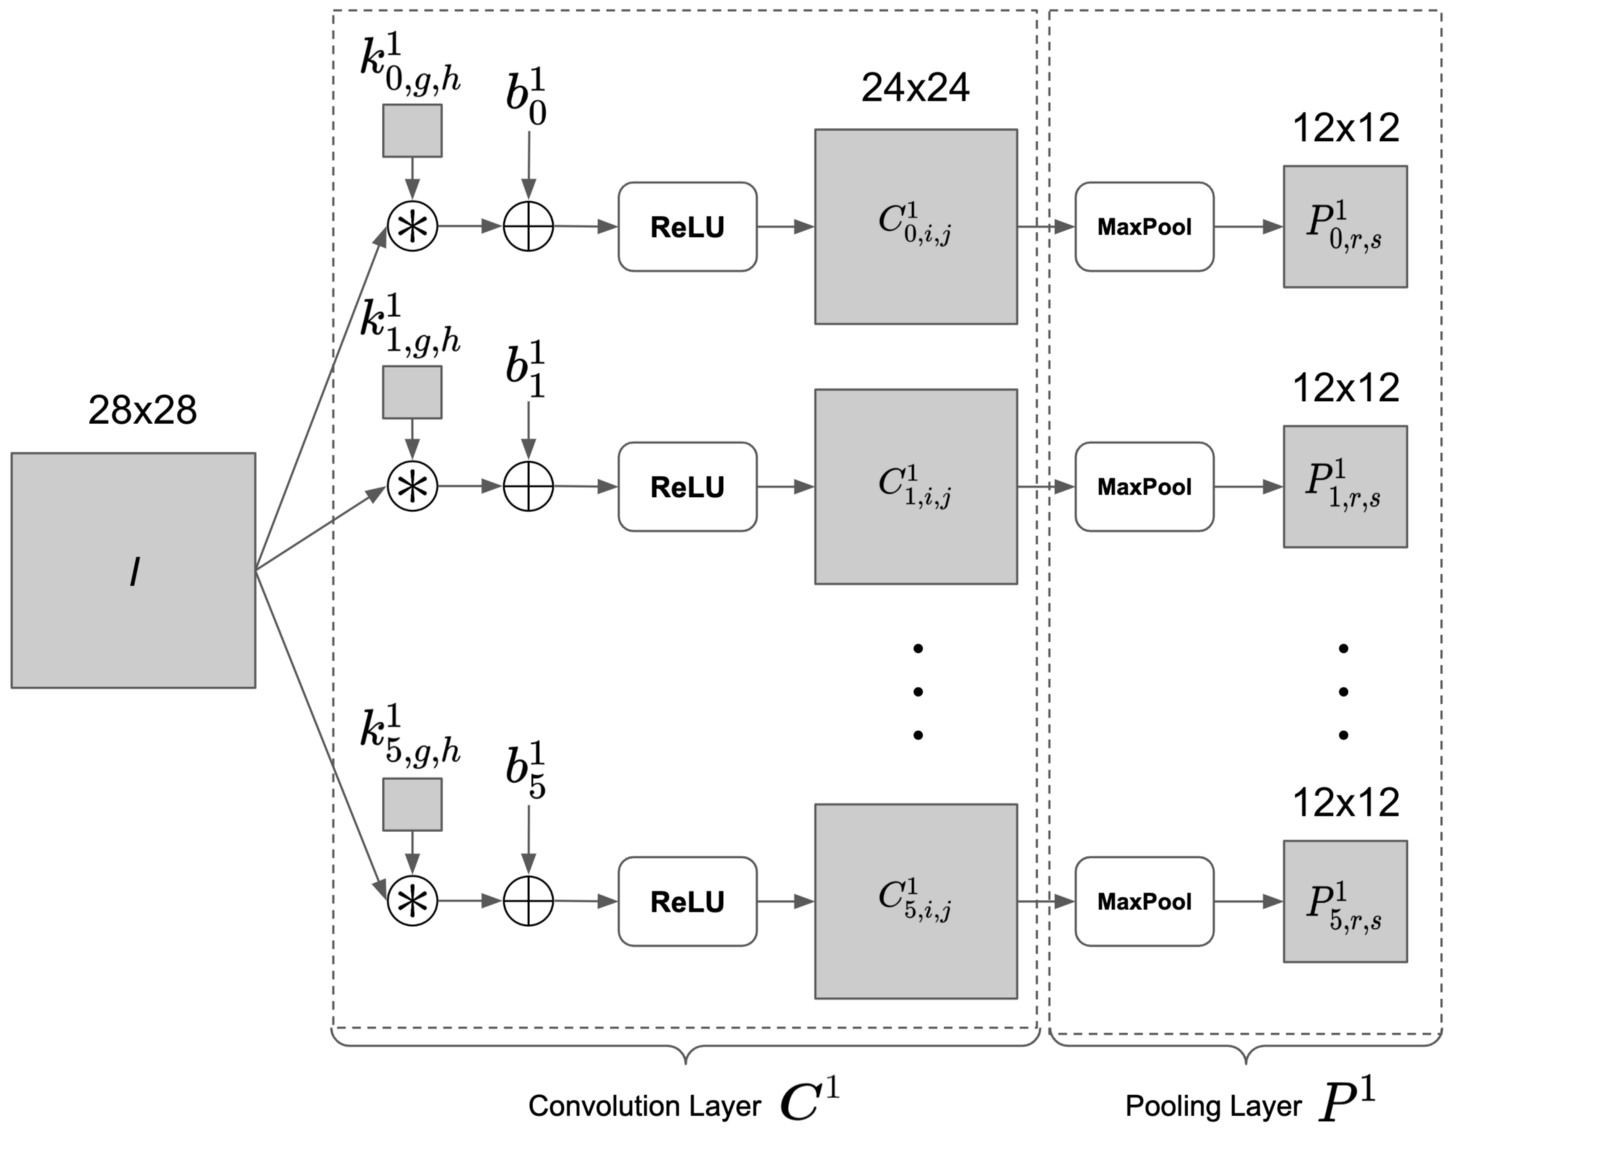
\includegraphics[width=11.6cm, height=8cm]{Architecture-part1.png}
    \caption{Detailed Architecture - part 1}
  \end{center}
\end{figure}
\begin{figure}[h]
  \begin{center}
    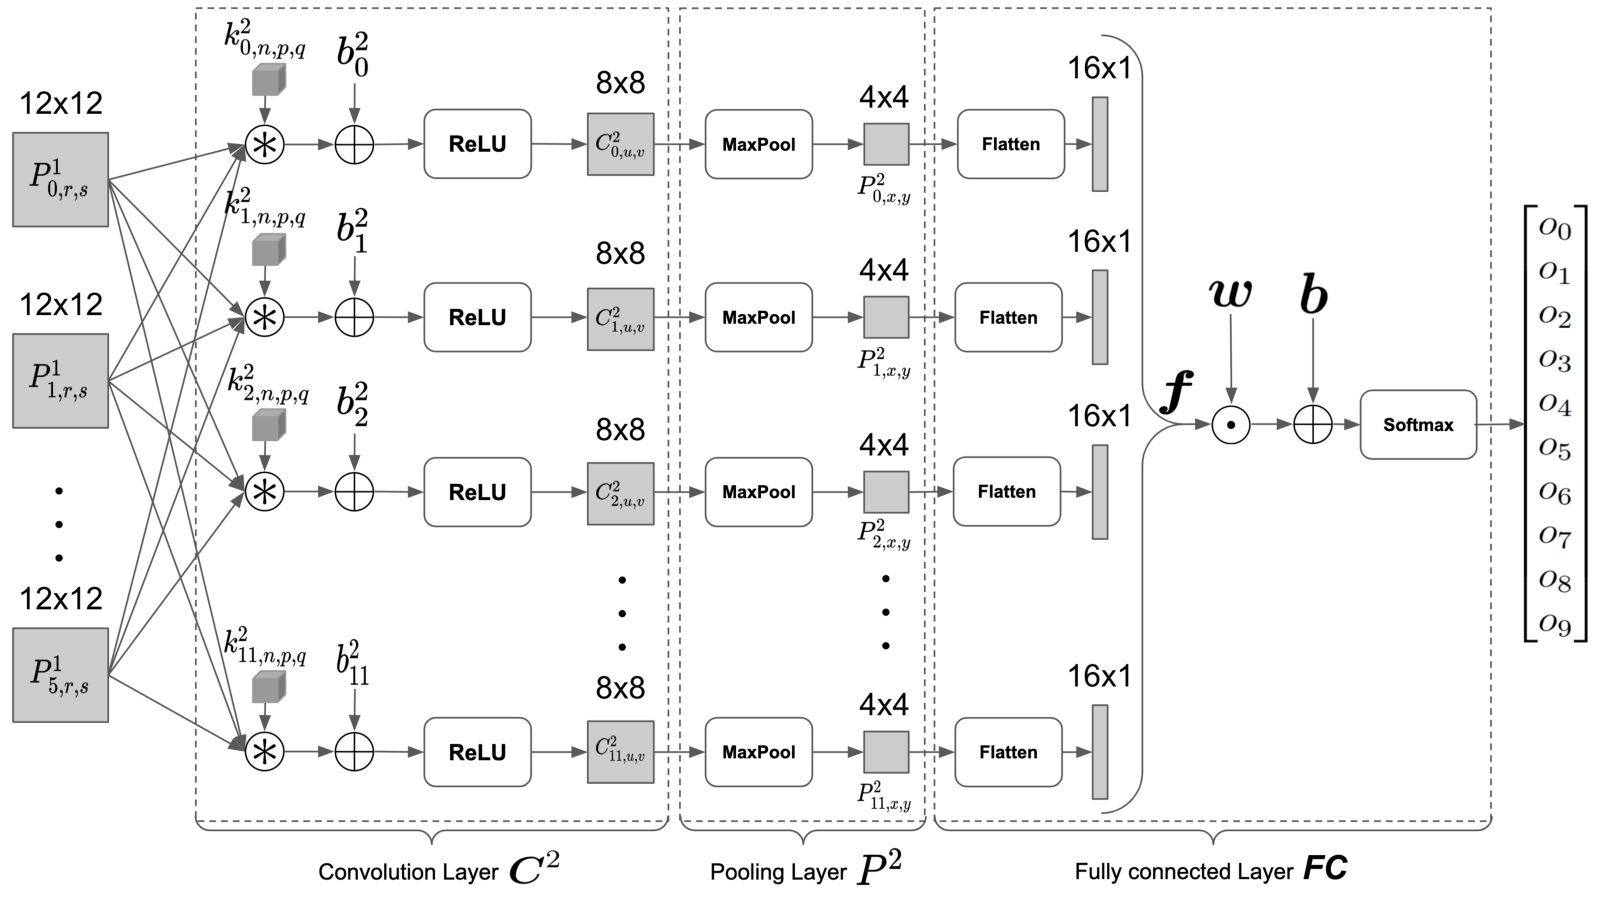
\includegraphics[width=15cm, height=8cm]{Architecture-part2.png}
    \caption{Detailed Architecture - part 2}
  \end{center}
\end{figure}\\
Like a standard Neural Network, training a Convolutional Neural Network consists of two phases \textbf{Feedforward} and \textbf{Backpropagation}.

\newpage
\section{Feedforward}
\medskip
By definition, the formula of \textbf{Feedforward} of each layer is represented as follows.
\subsection{Convolution Layer $\boldsymbol{C^1}$}

\begin{empheq}[box=\myyellowbox]{align}
\arraycolsep=0.05cm\def\arraystretch{1.0}
\begin{array}{ll}
S^{1}_{nij} = \sum\limits_{g=0}^{4}\sum\limits_{h=0}^{4}I_{g+i, h+j}k^{1}_{ngh} + b^{1}_{n}, \\[0.4cm]
C^{1}_{nij} = \text{ReLU}(S^{1}_{nij}) = \left\{
                \begin{array}{ll}
                  S^{1}_{nij} &\text{ if } S^{1}_{nij} > 0\\[0.2cm]
                  0           &\text{ if } S^{1}_{nij} \le 0
                \end{array}
              \right.\\[0.5cm]
n = 0, ..., 5;\thickspace i,j = 0, ..., 23 \label{eq1}
\end{array}
\end{empheq}
Where 6 kernels $k^1_{0gh}, ..., k^1_{5gh}$ are 2D arrays with size $5\times5$ and we assume that they were rotated $180\degree{}$ beforehand, and \textbf{stride} is set to $1$. $\boldsymbol{S^1}$ is the result of convolution between the grayscale image $\boldsymbol{I}$ and 6 kernels $k^1_{0gh}, ..., k^1_{5gh}$. Both $\boldsymbol{S^1}$ and $\boldsymbol{C^1}$ have the same size of $6\times24\times24$.

\subsection{Pooling Layer $\boldsymbol{P^1}$}
\begin{empheq}[box=\myyellowbox]{align}
\begin{array}{ll}
P^1_{nrs} = \max(C^{1}_{nij}), \thickspace i = 2r, 2r + 1, \thickspace j = 2s, 2s + 1, \\[0.2cm]
n = 0, ..., 5;\thickspace r,s = 0, ..., 11 \label{eq2}
\end{array}
\end{empheq}\\
Because we use pool size of $2\times2$, as a result $\boldsymbol{P^1}$ has a size of $6\times12\times12$.

\subsection{Convolution Layer $\boldsymbol{C^2}$}
\begin{empheq}[box=\myyellowbox]{align}
\arraycolsep=0.05cm\def\arraystretch{1.0}
\begin{array}{ll}
S^{2}_{muv} = \sum\limits_{n=0}^{5}\sum\limits_{p=0}^{4}\sum\limits_{q=0}^{4}P^{1}_{n,p+u, q+v}k^{2}_{mnpq} + b^{2}_{m}, \\[0.4cm]
C^{2}_{muv} = \text{ReLU}(S^{2}_{muv}) = \left\{
                \begin{array}{ll}
                  S^{2}_{muv} &\text{ if } S^{2}_{muv} > 0\\[0.2cm]
                  0           &\text{ if } S^{2}_{muv} \le 0
                \end{array}
              \right.\\[0.5cm]
m = 0, ..., 11;\thickspace u,v = 0, ..., 7 \label{eq3}
\end{array}
\end{empheq}\\
Where 12 kernels $k^2_{0npq}, ..., k^2_{11npq}$ are 3D arrays with size $6\times5\times5$ and we assume that they were rotated $180\degree{}$ beforehand, and \textbf{stride} is set to $1$. $\boldsymbol{S^2}$ is the result of convolution between $\boldsymbol{P^1}$ and 12 kernels $k^2_{0npq}, ..., k^2_{11npq}$. Both $\boldsymbol{S^2}$ and $\boldsymbol{C^2}$ have the same size of $12\times8\times8$.

\subsection{Pooling Layer $\boldsymbol{P^2}$}
\begin{empheq}[box=\myyellowbox]{align}
\begin{array}{ll}
P^2_{mxy} = \max(C^{2}_{muv}), \thickspace u = 2x, 2x + 1, \thickspace v = 2y, 2y + 1,\\[0.2cm]
m = 0, ..., 11;\thickspace x,y = 0, ..., 3 \label{eq4}
\end{array}
\end{empheq}

\subsection{Fully Connected Layer $\boldsymbol{FC}$}
\begin{empheq}[box=\myyellowbox]{align}
\begin{array}{ll}
\boldsymbol{f} = \text{flatten}(\boldsymbol{P^2})\\[0.4cm]
S_{i} = \sum\limits_{j=0}^{191}w_{ij}f_{j} + b_{i},\\[0.4cm]
O_{i} = \text{softmax}(S_{i}) = \frac{e^{S_{i}}}{\sum\limits_{k=0}^{9}e^{S_{k}}}, \\[0.2cm]
i = 0, ..., 9 \label{eq5}
\end{array}
\end{empheq}\\[-0.7cm]


\section{Backpropagation}
Like a standard Neural Network, in this Backpropagation phase, we also need to find optimal values of parameters so that the loss function $L$ is minimum. In Convolutional Neural Network, parameters are just kernels and biases ($\boldsymbol{k^1}$, $\boldsymbol{b^1}$, $\boldsymbol{k^2}$, and $\boldsymbol{b^2}$). Besides, the weight $\boldsymbol{w}$ and bias $\boldsymbol{b}$ are parameters too.\\[0.3cm]
Because in the Fully Connected Layer, we use \textbf{Softmax} as an activation function so the most suitable loss function should be a cross entropy (\url{https://en.wikipedia.org/wiki/Cross_entropy}).
\begin{empheq}[box=\myyellowbox]{align}
\begin{array}{ll}
L &= L(O_0, ..., O_9),\\
  &= L(O_{label}) \\
  &= -\ln(O_{label}), \thickspace label \in \{0, ..., 9\} \label{eq6}
\end{array}
\end{empheq}\\
where $label$ is the ground-truth value of the grayscale image $\boldsymbol{I}$, $\ln(O_{label})$ is the natural logarithm of $O_{label}$.\\[0.3cm]
To find optimal values of parameters, we will also apply the Stochastic Gradient Descent algorithm. First, we need to derive gradients of parameters in the Fully Connected Layer $\boldsymbol{FC}$, the Convolution Layer $\boldsymbol{C^1}$, and the Convolution Layer $\boldsymbol{C^2}$.

\medskip

\subsection{Deriving gradients of parameters in the Fully Connected Layer}

In the $\boldsymbol{FC}$ layer, we need to derive gradients $\frac{\partial{L}}{\partial{b_i}}$ and $\frac{\partial{L}}{\partial{w_{ij}}}$. From \eqref{eq6}, obviously we can say $L$ is a function of the variable $O_{label}$. In addition, from \eqref{eq5} we can also say $O_{label}$ is a function of multi-variables $S_i$ ($i = 0, ..., 9$) and for a specific $S_i$, we can say $S_i$ is a function of a specific $b_i$ and multi-variables $w_{ij}$ and $f_j$ ($j = 0, ..., 191$). Therefore, we can apply the chain rule to deriving gradients $\frac{\partial{L}}{\partial{b_i}}$ and $\frac{\partial{L}}{\partial{w_{ij}}}$ as follows.

\subsubsection{Deriving the gradient $\frac{\partial{L}}{\partial{b_i}}$}

Applying the chain rule, we can represent
\begin{equation}
\begin{aligned}
\frac{\partial{L}}{\partial{b_i}} &= \sum_{k=0}^9\frac{\partial{L}}{\partial{S_k}}\frac{\partial{S_k}}{\partial{b_i}},\thickspace i = 0, ..., 9 \label{eq7}
\end{aligned}
\end{equation}
From \eqref{eq5}, we can see obviously that
\begin{equation}
\begin{aligned}
\frac{\partial{S_k}}{\partial{b_i}} = \left\{
                                        \begin{array}{ll}
                                          1 \text{ if } k = i\\
                                          0 \text{ if } k \neq i
                                        \end{array}
                                      \right. \label{eq8}
\end{aligned}
\end{equation}
So we can reduce \eqref{eq7} as follows
\begin{equation}
\begin{aligned}
\frac{\partial{L}}{\partial{b_i}} &= \frac{\partial{L}}{\partial{S_i}},\thickspace i = 0, ..., 9 \label{eq9}
\end{aligned}
\end{equation}
Let's continue developing $\frac{\partial{L}}{\partial{S_i}}$ with the support of the chain rule.
\begin{equation}
\begin{aligned}
\frac{\partial{L}}{\partial{S_i}} &= \frac{\partial{L(O_{label})}}{\partial{O_{label}}}\frac{\partial{O_{label}}}{\partial{S_i}} \label{eq10}
\end{aligned}
\end{equation}
\begin{equation}
\begin{aligned}
\frac{\partial{L(O_{label})}}{\partial{O_{label}}} &= \frac{\partial{(-\ln(O_{label}))}}{\partial{O_{label}}}
                                                   &= -\frac{1}{O_{label}} \label{eq11}
\end{aligned}
\end{equation}
From \eqref{eq5} we have
\begin{equation}
\begin{aligned}
O_{label} &= \frac{e^{S_{label}}}{\sum\limits_{k=0}^{9}e^{S_{k}}} \label{eq12}
\end{aligned}
\end{equation}
Denote $T = \sum\limits_{k=0}^{9}e^{S_{k}}$, we can rewrite $O_{label}$ as follows
\begin{equation}
\begin{aligned}
O_{label} &= \frac{e^{S_{label}}}{T} = e^{S_{label}}T^{-1} \label{eq13}
\end{aligned}
\end{equation}
So we can develop
\begin{equation}
\begin{aligned}
\frac{\partial{O_{label}}}{\partial{S_i}} &= \frac{\partial{\big(e^{S_{label}}T^{-1}\big)}}{\partial{S_i}}, \thickspace i = 0, ..., 9\\ \label{eq14}
\end{aligned}
\end{equation}
Next, let's consider two cases:\\[0.5cm]
\textbf{\underline{Case 1:}} $i = label$, then we can rewrite \eqref{eq14} as follows
\begin{equation}
\begin{aligned}
\frac{\partial{O_{label}}}{\partial{S_{label}}} &= \frac{\partial{\big(e^{S_{label}}T^{-1}\big)}}{\partial{S_{label}}} \label{eq15}
\end{aligned}
\end{equation}
Denote $e^{S_{label}} = T - C_1$, where $C_1 = e^{S_0} + ... + e^{S_{label - 1}} + e^{S_{label + 1}} + ... + e^{S_{9}}$ and we can regard $C_1$ as a constant because $C_1$ is independent of $S_{label}$. Then,
\begin{equation}
\begin{aligned}
\frac{\partial{O_{label}}}{\partial{S_{label}}} &= \frac{\partial{\big((T - C_1)T^{-1}\big)}}{\partial{S_{label}}} \\
                                                &= \frac{\partial{\big(1 - C_1T^{-1}\big)}}{\partial{S_{label}}} \\
                                                &= -C_1\frac{\partial{T^{-1}}}{\partial{S_{label}}} \\
                                                &= -C_1\frac{\partial{T^{-1}}}{\partial{T}}\frac{\partial{T}}{\partial{S_{label}}} \\
                                                &= -C_1(-1T^{-2})\frac{\partial{T}}{\partial{S_{label}}} \\
                                                &= C_1T^{-2}\frac{\partial{T}}{\partial{S_{label}}} \label{eq16}
\end{aligned}
\end{equation}
\begin{equation}
\begin{aligned}
\frac{\partial{T}}{\partial{S_{label}}} &= \frac{\partial{(e^{S_{label}} + C_1)}}{\partial{S_{label}}} = \frac{\partial{e^{S_{label}}}}{\partial{S_{label}}} = e^{S_{label}} \label{eq17}
\end{aligned}
\end{equation}
Substitute \eqref{eq17} into \eqref{eq16},
\begin{equation}
\begin{aligned}
\frac{\partial{O_{label}}}{\partial{S_{label}}} &= C_1T^{-2}e^{S_{label}} \\
                                                &= (C_1T^{-1})(e^{S_{label}}T^{-1}) \\
                                                &= (T - e^{S_{label}})T^{-1}(e^{S_{label}}T^{-1}) \\
                                                &= (1 - e^{S_{label}}T^{-1})(e^{S_{label}}T^{-1}) \\
                                                &= (1 - O_{label})O_{label} \label{eq18}
\end{aligned}
\end{equation}
\textbf{\underline{Case 2:}} $i \neq label$, then we can regard $e^{S_{label}}$ as a constant and therefore,
\begin{equation}
\begin{aligned}
\frac{\partial{O_{label}}}{\partial{S_i}} &= e^{S_{label}}\frac{\partial{\big(T^{-1}\big)}}{\partial{S_i}} \\
                                          &= e^{S_{label}}\frac{\partial{\big(T^{-1}\big)}}{\partial{T}}\frac{{\partial{T}}}{\partial{S_i}} \\
                                          &= -e^{S_{label}}T^{-2}\frac{{\partial{T}}}{\partial{S_i}} \label{eq19}
\end{aligned}
\end{equation}
From \eqref{eq5}, we can represent $T = C_2 + e^{S_i}$, where $C_2 = e^{S_0} + ... + e^{S_{i - 1}} + e^{S_{i + 1}} + ... + e^{S_{9}}$ and we can regard $C_2$ as a constant because $C_2$ is independent of $S_i$. Then,
\begin{equation}
\begin{aligned}
\frac{{\partial{T}}}{\partial{S_i}} &= \frac{\partial{(C_2 + e^{S_i})}}{\partial{S_i}} = \frac{\partial{e^{S_i}}}{\partial{S_i}} = e^{S_i} \label{eq20}
\end{aligned}
\end{equation}
Substitute \eqref{eq20} into \eqref{eq19}, 
\begin{equation}
\begin{aligned}
\frac{\partial{O_{label}}}{\partial{S_i}} = -e^{S_{label}}T^{-2}e^{S_i} = -(e^{S_{label}}T^{-1})(e^{S_i}T^{-1}) = -O_{label}O_i \label{eq21}
\end{aligned}
\end{equation}\\[0.5cm]
Combine \textbf{Case 1} with \textbf{Case 2}, we have
\begin{equation}
\arraycolsep=0.05cm\def\arraystretch{1.0}
\begin{aligned}
\frac{\partial{O_{label}}}{\partial{S_{i}}} = \left\{
                                                \begin{array}{ll}
                                                  (1 - O_{label})O_{label} &\thickspace\text{ if } i = label\\[0.3cm]
                                                  -O_{label}O_i &\thickspace\text{ if } i \neq label
                                                \end{array}
                                               \right. ,\thickspace i = 0, ..., 9 \label{eq22}
\end{aligned}
\end{equation}
Substitute \eqref{eq22} and \eqref{eq11} into \eqref{eq10},
\begin{equation}
\arraycolsep=0.05cm\def\arraystretch{1.0}
\begin{aligned}
\frac{\partial{L}}{\partial{S_i}} &= \left\{
                                        \begin{array}{ll}
                                          O_{label} - 1 &\thickspace\text{ if } i = label\\[0.3cm]
                                          O_i &\thickspace\text{ if } i \neq label
                                        \end{array}
                                     \right. ,\thickspace i = 0, ..., 9 \label{eq23}
\end{aligned}
\end{equation}\\[0.5cm]
Denote \textbf{dLS} is an array of $\frac{\partial{L}}{\partial{S_i}}$, we can represent
\begin{empheq}[box=\myyellowbox]{align}
\textbf{dLS} = \begin{bmatrix}
\frac{\partial{L}}{\partial{S_0}}\\
.\\
.\\
.\\[0.2cm]
\frac{\partial{L}}{\partial{S_9}} 
\end{bmatrix}\label{eq24}
\end{empheq}
Substitute \eqref{eq23} into \eqref{eq9}, finally we obtain
\begin{equation}
\arraycolsep=0.05cm\def\arraystretch{1.0}
\frac{\partial{L}}{\partial{b_i}} = \left\{
                                        \begin{array}{ll}
                                          O_{label} - 1 &\thickspace\text{ if } i = label\\[0.3cm]
                                          O_i &\thickspace\text{ if } i \neq label
                                        \end{array}
                                     \right. ,\thickspace i = 0, ..., 9 \label{eq25}
\end{equation}
Denote \textbf{dLb} is an array of $\frac{\partial{L}}{\partial{b_i}}$, we can represent
\begin{empheq}[box=\myyellowbox]{align}
\textbf{dLb} = \begin{bmatrix}
  O_0\\
  .\\
  .\\
  .\\[0.2cm]
  O_{label} - 1\\
  .\\
  .\\
  .\\[0.2cm]
  O_9
\end{bmatrix}\label{eq26}
\end{empheq}



\subsubsection{Deriving the gradient $\frac{\partial{L}}{\partial{w_{ij}}}$}
Applying the chain rule, we can represent
\begin{equation}
\begin{aligned}
\frac{\partial{L}}{\partial{w_{ij}}} &= \sum_{k=0}^9\frac{\partial{L}}{\partial{S_k}}\frac{\partial{S_k}}{\partial{w_{ij}}},\thickspace i = 0, ..., 9, \thickspace j = 0, ..., 191 \label{eq27}
\end{aligned}
\end{equation}
From \eqref{eq5}, we can derive
\begin{equation}
\arraycolsep=0.05cm\def\arraystretch{1.0}
\begin{aligned}
\frac{\partial{S_k}}{\partial{w_{ij}}} = \frac{\partial{(\sum\limits_{t=0}^{191}w_{kt}f_{t} + b_{k})}}{\partial{w_{ij}}} = \left\{
                                        \begin{array}{ll}
                                          f_j &\thickspace\text{ if } k = i\\[0.3cm]
                                          0 &\thickspace\text{ if } k \neq i
                                        \end{array}
                                     \right. \label{eq28}
\end{aligned}
\end{equation}
So,
\begin{equation}
\begin{aligned}
\frac{\partial{L}}{\partial{w_{ij}}} &= \frac{\partial{L}}{\partial{S_i}}f_j,\thickspace i = 0, ..., 9, \thickspace j = 0, ..., 191 \label{eq29}
\end{aligned}
\end{equation}
Because we already calculated $\frac{\partial{L}}{\partial{S_i}}$ in \eqref{eq23}, so we can calculate $\frac{\partial{L}}{\partial{w_{ij}}}$ easily. Now denote \textbf{dLw} is a 2D array of $\frac{\partial{L}}{\partial{w_{ij}}}$, we can represent
\begin{empheq}[box=\myyellowbox]{align}
\textbf{dLw} = \begin{bmatrix}
  \frac{\partial{L}}{\partial{S_0}}f_0 \thickspace.................................................\thickspace \frac{\partial{L}}{\partial{S_0}}f_{191}\\
  ..................................................................\\
  ..................................................................\\
  ..................................................................\\[0.2cm]
  \frac{\partial{L}}{\partial{S_9}}f_0 \thickspace.................................................\thickspace \frac{\partial{L}}{\partial{S_9}}f_{191}
\end{bmatrix}\label{eq30}
\end{empheq}

\subsection{Deriving gradients of parameters in the Convolution Layer $\boldsymbol{C^2}$}
For a specific $b^2_m$ (or $k^2_{mnpq}$), from the equations in the \textbf{Feedforward} section, we can see obviously that every $S^2_{muv}$ is a function of 301 variables ($P^1_{n, p+u, q+v}, k^2_{mnpq}, b^2_{m}$) ($n = 0,...,5,\thickspace p = 0,...,4,\thickspace q = 0,...,4$), and every $C^2_{muv}$ is a function of one variable $S^2_{muv}$, and every $P^2_{mxy}$ is a function of 4 variables $C^2_{muv}$ ($u = 2x, 2x + 1,\thickspace v = 2y, 2y + 1$), and every $f_k$ ($k = 16m + 4x + y$) is equal to one $P^2_{mxy}$. If the variable $b^2_m$ (or $k^2_{mnpq}$) changes a bit, it will affect all $S^2_{muv}$ ($u = 0,...,7,\thickspace v = 0,...,7$) and then like the domino effect, all $C^2_{muv}$ and all $P^2_{mxy}$ will be affected. Next, only 16 $f_k$ elements ($k = 16m, 16m + 15$) will be affected. Next, all $S_i$ ($i = 0, ..., 9$) will be effected. Finally, the change will cause $L$ changes accordingly. Based on these nested relationships and applying the chain rule, we can derive $\frac{\partial{L}}{\partial{b^2_m}}$ and $\frac{\partial{L}}{\partial{k^2_{mnpq}}}$ as follows.

\subsubsection{Deriving the gradient $\frac{\partial{L}}{\partial{b^2_m}}$ $(m = 0, ..., 11)$}
\begin{equation}
\begin{aligned}
\frac{\partial{L}}{\partial{b^2_{m}}} = \sum\limits_{u = 0}^{7}\sum\limits_{v = 0}^{7}\frac{\partial{L}}{\partial{S^2_{muv}}}\frac{\partial{S^2_{muv}}}{\partial{b^2_{m}}}\label{eq31}
\end{aligned}
\end{equation}

\begin{equation}
\begin{aligned}
\frac{\partial{L}}{\partial{S^2_{muv}}} = \frac{\partial{L}}{\partial{C^2_{muv}}}\frac{\partial{C^2_{muv}}}{\partial{S^2_{muv}}} \label{eq32}
\end{aligned}
\end{equation}
Let's calculate $\frac{\partial{L}}{\partial{C^2_{muv}}}$.\\
Because of how \textbf{MaxPool} (pool size = $2\times2$) works (please review \url{https://victorzhou.com/blog/intro-to-cnns-part-2/#4-backprop-max-pooling}), one specific $C^2_{muv}$ always belongs to a certain block of 4 elements (the $C^2_{muv}$ and 3 other elements of the 3D array $\boldsymbol{C^2}$) and it may or may not be the maximum element out of 4 elements. Considering two following cases:\\[0.5cm]
\underline{\textbf{Case 1:}} $C^2_{muv}$ is the maximum element out of 4 elements. Denote $u = u_{max}$, $v = v_{max}$.\\ 
Then, $C^2_{muv} = C^2_{mu_{max}v_{max}}$ and $P^2_{mxy} = C^2_{mu_{max}v_{max}}$ ($x = \text{floor}(u_{max} / 2),\thickspace y = \text{floor}(v_{max} / 2)$).\\
\begin{equation}
\begin{aligned}
\frac{\partial{L}}{\partial{C^2_{muv}}} = \frac{\partial{L}}{\partial{C^2_{mu_{max}v_{max}}}} = \frac{\partial{L}}{\partial{P^2_{mxy}}} \label{eq33}
\end{aligned}
\end{equation}
Furthermore, $f_k = P^2_{mxy}$ ($k = 16m + 4x + y$). It follows that 
\begin{equation}
\begin{aligned}
\frac{\partial{L}}{\partial{C^2_{mu_{max}v_{max}}}} = \frac{\partial{L}}{\partial{P^2_{mxy}}} = \frac{\partial{L}}{\partial{f_k}} \label{eq34}
\end{aligned}
\end{equation}
Let's calculate $\frac{\partial{L}}{\partial{f_k}}$:
\begin{equation}
\begin{aligned}
\frac{\partial{L}}{\partial{f_k}} = \sum\limits_{i = 0}^{9}\frac{\partial{L}}{\partial{S_i}}\frac{\partial{S_i}}{\partial{f_k}} \label{eq35}
\end{aligned}
\end{equation}
From \eqref{eq5}, we can derive
\begin{equation}
\begin{aligned}
\frac{\partial{S_i}}{\partial{f_k}} = w_{ik} \label{eq36}
\end{aligned}
\end{equation}
Substitute \eqref{eq36} into \eqref{eq35},
\begin{equation}
\begin{aligned}
\frac{\partial{L}}{\partial{f_k}} = \sum\limits_{i = 0}^{9}\frac{\partial{L}}{\partial{S_i}}w_{ik} \label{eq37}
\end{aligned}
\end{equation}
Denote \textbf{dLf} is a 1D array of $\frac{\partial{L}}{\partial{f_k}}$ with shape = (192), then we can represent
\begin{empheq}[box=\myyellowbox]{equation}
\textbf{dLf} = \textbf{w}^T \cdot \textbf{dLS} \label{eq38}
\end{empheq}
Denote \textbf{dLP2} is a 3D array of $\frac{\partial{L}}{\partial{\boldsymbol{P^2}}}$ with shape = $\boldsymbol{P^2}$.shape = $(12, 4, 4)$, then we can represent
\begin{empheq}[box=\myyellowbox]{equation}
\textbf{dLP2} = \textbf{dLf}.\text{reshape}(\boldsymbol{P^2}.\text{shape}) \label{eq39}
\end{empheq}
\\[0.5cm]
\underline{\textbf{Case 2:}} $C^2_{muv}$ is not the maximum element out of 4 elements. Then, if $C^2_{muv}$ changes a super small quantity, that change will not affect $P^2_{mxy}$ ($x = \text{floor}(u / 2),\thickspace y = \text{floor}(v / 2)$) at all. For example, given the following block of 4 $C^2_{muv}$ elements (as shown in Figure 4)\\
\begin{figure}[h]
  \begin{center}
    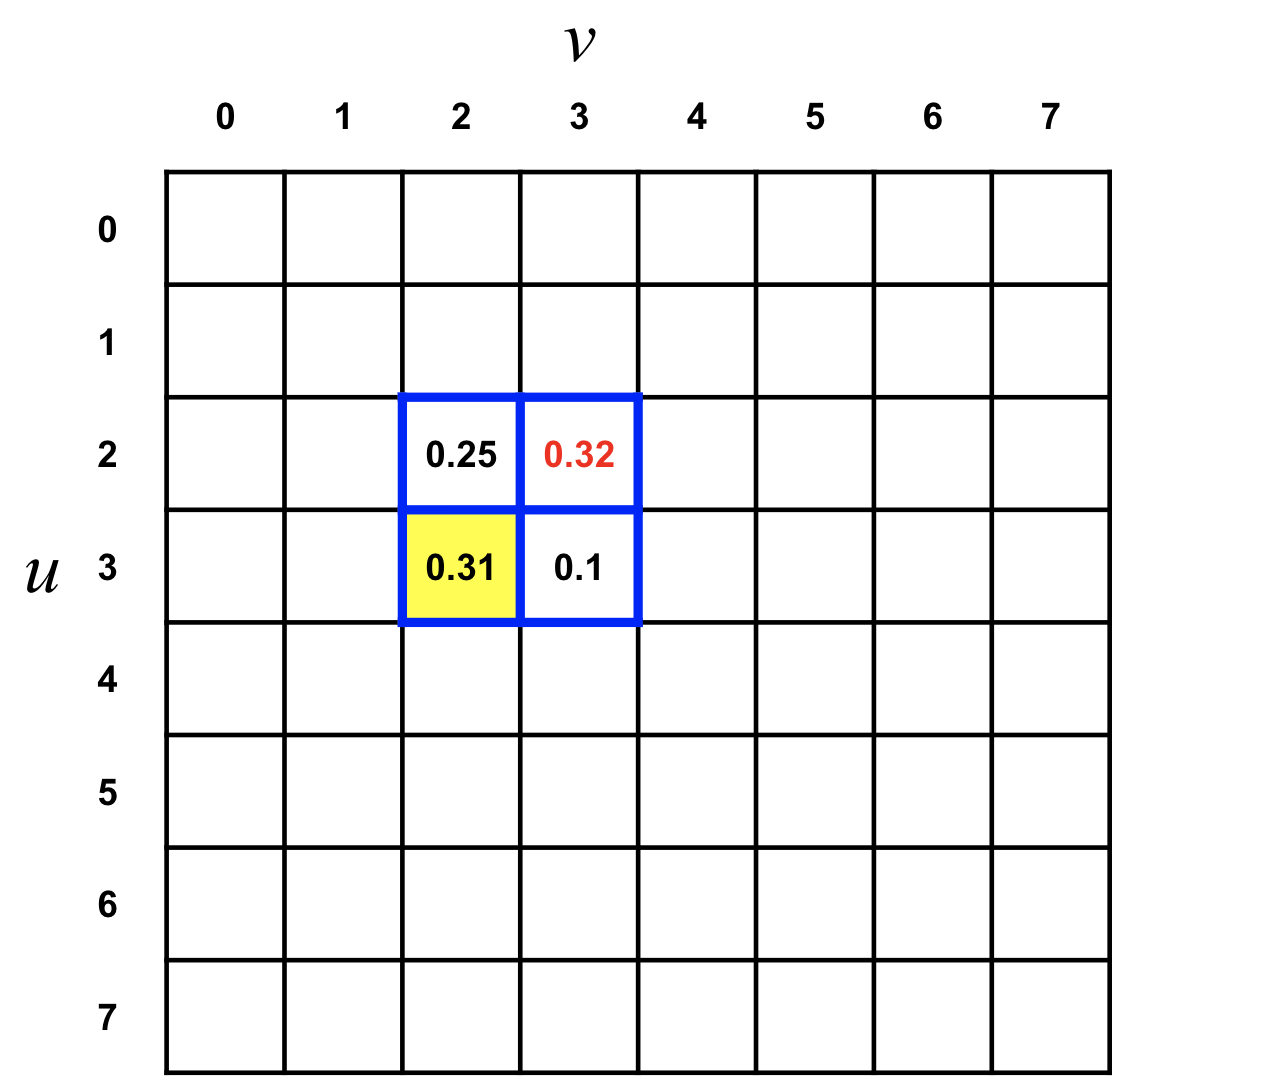
\includegraphics[width=9cm, height=8cm]{C2.png}
    \caption{A sample $\boldsymbol{C^2}$[m]}
  \end{center}
  \label{fig:maxpool}
\end{figure}\\
Suppose that $u = 3, v = 2$, then $C^2_{muv} = 0.31$ (the yellow cell) and obviously we have $u_{max} = 2, v_{max} = 3$, and $C^2_{mu_{max}v_{max}} = 0.32$. So $x = \text{floor}(u / 2) = \text{floor}(3 / 2) = 1, y = \text{floor}(v / 2) = \text{floor}(2 / 2) = 1$, and thus $P^2_{mxy} = P^2_{m11} = C^2_{mu_{max}v_{max}} = 0.32$. If we increase $C^2_{muv}$ by $10^{-9}$, that is $C^2_{muv} = C^2_{muv} + 10^{-9} = 0.31 + 10^{-9}$. The new $C^2_{muv}$ still doesn't affect the $P^2_{mxy}$ at all. As a result, the change doesn't affect the loss function $L$. From this observation, we can state that in this case
\begin{equation}
\begin{aligned}
\frac{\partial{L}}{\partial{C^2_{muv}}} = 0  \label{eq40}
\end{aligned}
\end{equation}
Combining \textbf{Case 1} with \textbf{Case 2}, we can express
\begin{equation}
\begin{aligned}
\frac{\partial{L}}{\partial{C^2_{muv}}} = \left\{
                                            \begin{array}{ll}
                                              \frac{\partial{L}}{\partial{P^2_{mxy}}},\thickspace \big(x = \text{floor}(u/2), \thickspace y = \text{floor}(v/2)\big) \text{ if } C^2_{muv} \text{ is the maximum element}\\ \text{out of 4 elements. } \\[0.3cm]
                                              0 \text{ otherwise }
                                            \end{array}
                                          \right. \label{eq41}
\end{aligned}
\end{equation}
Denote \textbf{dLC2} is a 3D array of $\frac{\partial{L}}{\partial{C^2_{muv}}}$ elements $\Big(\textbf{dLC2}[m, u, v] = \frac{\partial{L}}{\partial{C^2_{muv}}}\Big)$, with shape = $\boldsymbol{C^2}$.shape. We can form a procedure to calculate $\textbf{dLC2}[m, u, v]$ as follows:
\begin{itemize}
  \item In the \textbf{Feedforward} phase, we cache $(m, u_{max}, v_{max})$ into a 3D array \textbf{I2} (with shape = $\boldsymbol{P^2}$.shape) like this:
    \begin{empheq}[box=\myyellowbox]{equation}
      \textbf{I2}[m,x,y] = \begin{bmatrix}u_{max}\\ v_{max}\end{bmatrix},\thickspace x = u_{max} / 2, \thickspace y = v_{max} / 2 \label{eq42}
    \end{empheq}
  \item Calculate \textbf{dLP2} using equations \eqref{eq38} and \eqref{eq39}.
  \item Initialize $\textbf{dLC2} = 0$ (all \textbf{dLC2}'s elements are zero).
  \item Loop through all triple $(m,x,y)$, $m = 0, ..., 11$; $x,y = 0, ..., 3$:
    \begin{empheq}[box=\myyellowbox]{align}
    \begin{array}{ll}
      \text{Retrieve } u_{max}, v_{max} \text{ from } \textbf{I2}[m,x,y],\\[0.3cm]
      \textbf{dLC2}[m, u_{max}, v_{max}] = \textbf{dLP2}[m, x, y]
    \end{array} \label{eq43}
    \end{empheq}
\end{itemize}
So every $\textbf{dLC2}[m, u, v] = \frac{\partial{L}}{\partial{C^2_{muv}}}$ is calculated.\\[0.5cm]
Next, denote \textbf{dC2S2} is a 3D array of $\frac{\partial{C^2_{muv}}}{\partial{S^2_{muv}}}$ elements $\Big(\textbf{dC2S2}[m,u,v] = \frac{\partial{C^2_{muv}}}{\partial{S^2_{muv}}}\Big)$, then just in the \textbf{Feedforward} phase we can also calculate \textbf{dC2S2}$[m,u,v]$ using \eqref{eq3} as follows:
\begin{empheq}[box=\myyellowbox]{equation}
\textbf{dC2S2}[m,u,v] = \frac{\partial{C^2_{muv}}}{\partial{S^2_{muv}}} = \left\{
                          \begin{array}{ll}
                            1 \text{ if } S^2_{muv} > 0\\[0.3cm]
                            0 \text{ if } S^2_{muv} \le 0
                          \end{array}
                        \right. \label{eq44}
\end{empheq}
So we can rewrite \eqref{eq32} as follows:
\begin{empheq}[box=\myyellowbox]{equation}
\textbf{dLS2}[m,u,v] = \frac{\partial{L}}{\partial{S^2_{muv}}} = \textbf{dLC2}[m,u,v]\textbf{dC2S2}[m,u,v] \label{eq45}
\end{empheq}
where, \textbf{dLS2} is a 3D array of $\frac{\partial{L}}{\partial{S^2_{muv}}}$ elements.\\[0.5cm]
From \eqref{eq3}, we can calculate 
\begin{equation}
\begin{aligned}
  \frac{\partial{S^2_{muv}}}{\partial{b^2_{m}}} = 1 \label{eq46}
\end{aligned}
\end{equation}
Finally, substitute \eqref{eq46} and \eqref{eq45} into \eqref{eq31}, we obtain
\begin{empheq}[box=\myyellowbox]{equation}
\frac{\partial{L}}{\partial{b^2_{m}}} = \sum\limits_{u = 0}^{7}\sum\limits_{v = 0}^{7}\textbf{dLS2}[m,u,v] \label{eq47}
\end{empheq}

\subsubsection{Deriving the gradient $\frac{\partial{L}}{\partial{k^2_{mnpq}}}$}
\begin{equation}
\begin{aligned}
\frac{\partial{L}}{\partial{k^2_{mnpq}}} = \sum\limits_{u = 0}^{7}\sum\limits_{v = 0}^{7}\frac{\partial{L}}{\partial{S^2_{muv}}}\frac{\partial{S^2_{muv}}}{\partial{k^2_{mnpq}}}\label{eq48}
\end{aligned}
\end{equation}
From \eqref{eq3}, we can calculate 
\begin{equation}
\begin{aligned}
  \frac{\partial{S^2_{muv}}}{\partial{k^2_{mnpq}}} = P^1_{n,p+u,q+v} \label{eq49}
\end{aligned}
\end{equation}
Substitute \eqref{eq49} into \eqref{eq48}, we obtain
\begin{empheq}[box=\myyellowbox]{equation}
\frac{\partial{L}}{\partial{k^2_{mnpq}}} = \sum\limits_{u = 0}^{7}\sum\limits_{v = 0}^{7}\frac{\partial{L}}{\partial{S^2_{muv}}}P^1_{n,p+u,q+v} \label{eq50}
\end{empheq}

\subsection{Deriving gradients of parameters in the Convolution Layer $\boldsymbol{C^1}$}

\subsubsection{Deriving the gradient $\frac{\partial{L}}{\partial{b^1_n}}$ $(n = 0, ..., 5)$}
\begin{equation}
\begin{aligned}
\frac{\partial{L}}{\partial{b^1_{n}}} = \sum\limits_{i = 0}^{23}\sum\limits_{j = 0}^{23}\frac{\partial{L}}{\partial{S^1_{nij}}}\frac{\partial{S^1_{nij}}}{\partial{b^1_{n}}}\label{eq51}
\end{aligned}
\end{equation}

\begin{equation}
\begin{aligned}
\frac{\partial{L}}{\partial{S^1_{nij}}} = \frac{\partial{L}}{\partial{C^1_{nij}}}\frac{\partial{C^1_{nij}}}{\partial{S^1_{nij}}} \label{eq52}
\end{aligned}
\end{equation}

\begin{equation}
\begin{aligned}
\frac{\partial{L}}{\partial{C^1_{nij}}} = \left\{
                                            \begin{array}{ll}
                                              \frac{\partial{L}}{\partial{P^1_{nrs}}},\thickspace \big(r = \text{floor}(i/2), \thickspace s = \text{floor}(j/2)\big) \text{ if } C^1_{nij} \text{ is the maximum element}\\ \text{out of 4 elements. } \\[0.3cm]
                                              0 \text{ otherwise }
                                            \end{array}
                                          \right. \label{eq53}
\end{aligned}
\end{equation}
Let's calculate $\frac{\partial{L}}{\partial{P^1_{nrs}}}$.\\
From \eqref{eq3} and the architecture diagrams, we can see that a specific $P^1_{nrs}$ may affect all $S^2_{muv}$. Therefore,
\begin{equation}
\begin{aligned}
\frac{\partial{L}}{\partial{P^1_{nrs}}} = \sum\limits_{m = 0}^{11}\sum\limits_{u = 0}^{7}\sum\limits_{v = 0}^{7}\frac{\partial{L}}{\partial{S^2_{muv}}}\frac{\partial{S^2_{muv}}}{\partial{P^1_{nrs}}} \label{eq54}
\end{aligned}
\end{equation}
We only need to calculate $\frac{\partial{S^2_{muv}}}{\partial{P^1_{nrs}}}$ because $\frac{\partial{L}}{\partial{S^2_{muv}}}$ was already calculated in \eqref{eq45}.\\
From \eqref{eq3}, we see that for a specific triple $(m, u, v)$, there is a 3D region of $P^1_{nrs}$ elements ($n = 0,...,5$, $r = u,...,u + 4$, $s = v,...,v + 4$) contributing to $S^2_{muv}$, and $\frac{\partial{S^2_{muv}}}{\partial{P^1_{nrs}}} = k^2_{mnpq}, \thickspace p = r - u, \thickspace q = s - v$. If an element $P^1_{nrs}$ is outside that 3D region, it doesn't contribute to $S^2_{muv}$, and therefore $\frac{\partial{S^2_{muv}}}{\partial{P^1_{nrs}}} = 0$. So denote \textbf{dS2P1} is a 6D array of $\frac{\partial{S^2_{muv}}}{\partial{P^1_{nrs}}}$ elements $\Big(\textbf{dS2P1}[n, r, s, m, u, v] = \frac{\partial{S^2_{muv}}}{\partial{P^1_{nrs}}}\Big)$ with \textbf{dS2P1}.shape = $\boldsymbol{P^1}$.shape + $\boldsymbol{C^2}$.shape = $(6, 12, 12, 12, 8, 8)$, we can calculate $\textbf{dS2P1}[n, r, s, m, u, v]$ just in the \textbf{Feedforward} phase using the following procedure:\\
\begin{itemize}
  \item Initialize $\textbf{dS2P1} = 0$
  \item Loop through all triple $(m, u, v), \thickspace m = 0, ..., 11, \thickspace u = 0, ..., 7, \thickspace v = 0, ..., 7$:
  \begin{empheq}[box=\myyellowbox]{equation}
    \textbf{dS2P1}[0:6, u:(u + 5), v:(v + 5), m, u, v] = \boldsymbol{k^2}[m] \label{eq55}
  \end{empheq}
\end{itemize}
Note that in \eqref{eq55}, \textbf{dS2P1} and $\boldsymbol{k^2}$ are Numpy arrays and $\boldsymbol{k^2}[m]$ is a 3D array of $k^2_{mnpq}$, $n = 0, ..., 5;\thickspace p,q = 0, ..., 4$.\\[0.5cm]
Substitute \eqref{eq45} and $\textbf{dS2P1}[n, r, s, m, u, v]$ calculated above into \eqref{eq54}, we obtain
\begin{equation}
\begin{aligned}
\frac{\partial{L}}{\partial{P^1_{nrs}}} = \sum\limits_{m = 0}^{11}\sum\limits_{u = 0}^{7}\sum\limits_{v = 0}^{7}\textbf{dLS2}[m,u,v]\textbf{dS2P1}[n, r, s, m, u, v] \label{eq56}
\end{aligned}
\end{equation}\\[0.5cm]
Denote \textbf{dLP1} is a 3D array of $\frac{\partial{L}}{\partial{P^1_{nrs}}}$ elements $\Big(\textbf{dLP1}[n,r,s] = \frac{\partial{L}}{\partial{P^1_{nrs}}}\Big)$ and \textbf{dLC1} is a 3D array of $\frac{\partial{L}}{\partial{C^1_{nij}}}$ elements $\Big(\textbf{dLC1}[n,i,j] = \frac{\partial{L}}{\partial{C^1_{nij}}}\Big)$. And, if just in the \textbf{Feedforward} phase, we cache triple $(n, i_{max}, j_{max})$ at which $C^1_{ni_{max}j_{max}}$ is the maximum element out of 4 elements into a 3D array \textbf{I1} 
    \begin{empheq}[box=\myyellowbox]{equation}
      \textbf{I1}[n,r,s] = \begin{bmatrix}i_{max}\\ j_{max}\end{bmatrix},\thickspace r = i_{max} / 2, \thickspace s = j_{max} / 2 \label{eq57}
    \end{empheq}
Then we can calculate $\textbf{dLC1}[n,i,j]$ as follows:
\begin{itemize}
  \item Initialize $\textbf{dLC1} = 0$.
  \item Loop through all triple $(n,r,s)$, $n = 0, ..., 5$; $r,s = 0, ..., 11$:
    \begin{empheq}[box=\myyellowbox]{align}
    \begin{array}{ll}
      \text{Retrieve } i_{max}, j_{max} \text{ from } \textbf{I1}[n,r,s],\\[0.3cm]
      \textbf{dLC1}[n, i_{max}, j_{max}] = \textbf{dLP1}[n, r, s]
    \end{array} \label{eq58}
    \end{empheq}
\end{itemize}
Next, denote \textbf{dC1S1} is a 3D array of $\frac{\partial{C^1_{nij}}}{\partial{S^1_{nij}}}$ elements $\Big(\textbf{dC1S1}[n,i,j] = \frac{\partial{C^1_{nij}}}{\partial{S^1_{nij}}}\Big)$, then just in the \textbf{Feedforward} phase we can also calculate \textbf{dC1S1}$[n,i,j]$ using \eqref{eq1} as follows:
\begin{empheq}[box=\myyellowbox]{equation}
\textbf{dC1S1}[n,i,j] = \frac{\partial{C^1_{nij}}}{\partial{S^1_{nij}}} = \left\{
                          \begin{array}{ll}
                            1 \text{ if } S^1_{nij} > 0\\[0.3cm]
                            0 \text{ if } S^2_{nij} \le 0
                          \end{array}
                        \right. \label{eq59}
\end{empheq}
Substitute the calculated $\textbf{dLC1}[n,i,j] = \frac{\partial{L}}{\partial{C^1_{nij}}}$ and $\textbf{dC1S1}[n,i,j] = \frac{\partial{C^1_{nij}}}{\partial{S^1_{nij}}}$ into \eqref{eq52}, we obtain
\begin{equation}
\begin{aligned}
\frac{\partial{L}}{\partial{S^1_{nij}}} = \textbf{dLC1}[n,i,j]\textbf{dC1S1}[n,i,j] \label{eq60}
\end{aligned}
\end{equation}\\[0.5cm]
Next, from \eqref{eq1}, we can see obviously that
\begin{equation}
\begin{aligned}
\frac{\partial{S^1_{nij}}}{\partial{b^1_{n}}} = 1 \label{eq61}
\end{aligned}
\end{equation}
Finally, substitute \eqref{eq61} and \eqref{eq60} into \eqref{eq51}, we obtain
\begin{empheq}[box=\myyellowbox]{equation}
\frac{\partial{L}}{\partial{b^1_{n}}} = \sum\limits_{i = 0}^{23}\sum\limits_{j = 0}^{23}\textbf{dLC1}[n,i,j]\textbf{dC1S1}[n,i,j] \label{eq62}
\end{empheq}

\subsubsection{Deriving the gradient $\frac{\partial{L}}{\partial{k^1_{ngh}}}$ $(n = 0, ..., 5;\thickspace g,h = 0, ..., 4)$}
\begin{equation}
\begin{aligned}
\frac{\partial{L}}{\partial{k^1_{ngh}}} = \sum\limits_{i = 0}^{23}\sum\limits_{j = 0}^{23}\frac{\partial{L}}{\partial{S^1_{nij}}}\frac{\partial{S^1_{nij}}}{\partial{k^1_{ngh}}} \label{eq63}
\end{aligned}
\end{equation}
$\frac{\partial{L}}{\partial{S^1_{nij}}}$ was calculated in \eqref{eq60}. So the rest of work is to calculate $\frac{\partial{S^1_{nij}}}{\partial{k^1_{ngh}}}$ and we can calculate it easily using \eqref{eq1}:
\begin{equation}
\begin{aligned}
\frac{\partial{S^1_{nij}}}{\partial{k^1_{ngh}}} = I_{n,g+i,h+j} \label{eq64}
\end{aligned}
\end{equation}
Substitute \eqref{eq64} into \eqref{eq63}, we obtain
\begin{equation}
\begin{aligned}
\frac{\partial{L}}{\partial{k^1_{ngh}}} = \sum\limits_{i = 0}^{23}\sum\limits_{j = 0}^{23}\frac{\partial{L}}{\partial{S^1_{nij}}}I_{n,g+i,h+j} \label{eq65}
\end{aligned}
\end{equation}

\subsection{Update parameters}
\begin{empheq}[box=\myyellowbox]{equation}
\begin{array}{ll}
k^1_{ngh} = k^1_{ngh} - \eta\frac{\partial{L}}{\partial{k^1_{ngh}}},\thickspace n = 0, ..., 5;\thickspace g,h = 0, ..., 4,\\[0.3cm]
b^1_n = b^1_n - \eta\frac{\partial{L}}{\partial{b^1_n}},\thickspace n = 0, ..., 5,\\[0.5cm]
k^2_{mnpq} = k^2_{mnpq} - \eta\frac{\partial{L}}{\partial{k^2_{mnpq}}},\thickspace m = 0, ..., 11, \thickspace n = 0, ..., 5;\thickspace p,q = 0, ..., 4,\\[0.3cm]
b^2_m = b^2_m - \eta\frac{\partial{L}}{\partial{b^2_m}},\thickspace m = 0, ..., 11,\\[0.5cm]
w_{ij} = w_{ij} - \eta\frac{\partial{L}}{\partial{w_{ij}}},\thickspace i = 0, ..., 9,\thickspace j = 0, ..., 191,\\[0.3cm]
b_i = b_i - \eta\frac{\partial{L}}{\partial{b_i}},\thickspace i = 0, ..., 9. \label{eq66}
\end{array}
\end{empheq}
Where $\eta$ is the learning rate.

\end{document}